\documentclass{article}

\usepackage{listings}
\usepackage{color}
\usepackage{courier}
\usepackage{amsmath}
\usepackage{graphicx}
\usepackage{float}
\usepackage[spanish]{babel}
\usepackage[utf8]{inputenc}
\usepackage{mleftright}
\usepackage{csvsimple}

\newcommand{\lnn}[1]{%
	\ln\left(#1\right)%
}

\newcommand{\lnb}[1]{%
	\ln\mleft(#1\mright)%
}


\title{PEC III - Física Computacional II}
\date{26-11-2023}
\author{Arturo Felipe Albacete Fernández}



\lstset{
	basicstyle=\footnotesize\ttfamily,
	breaklines=true,
	frame=tb,
	tabsize=4,
	columns=fixed,
	showstringspaces=false,
	showtabs=false,
	keepspaces,
	commentstyle=\color{red},
	keywordstyle=\color{blue}
}
\lstset{frame=single}


\begin{document}

% titulo
\maketitle
\newpage

% TOC
\tableofcontents
\newpage

% intro
%
% Introducción
%

\section{Introducción}

\paragraph{}
En este documento se encuentran redactadas las respuestas a la Prueba de Evaluación Continua 3. Se ha utilizado Python como lenguaje de programación y LaTeX para generar este documento.

\subsection{Sobre este documento}

\subparagraph{Estructura}
A cada pregunta se le ha dedicado una sección, en la que se intenta responder a los distintos puntos de la cuestión así como una explicación del código relacionado a la solución de dicha pregunta. En algunos casos, si una pregunta ya ha sido contestada en un apartado anterior, lo anotaré. 

\subparagraph{Código}
El código para esta (y otras PECs) lo estaré publicando en un repositorio git. Se puede acceder via:

\begin{lstlisting}[language=bash]
	git clone https://gitlab.com/aalbacetef/fisica-comp-II.git entrega-aalbacetef-fc-ii
\end{lstlisting}


Si se desea, puedo enviar por correo electrónico el código del proyecto en archivo comprimido (tar/rar/zip/7z/etc...).

Gran parte del código lo he puesto en el apéndice, pero recomiendo ver el repositorio git para poder leerlo más cómodamente.


\subsection{Ejecutar el código}

Para ejecutar el código es necesario tener Python instalado. He facilitado esto con el uso de Docker y un Makefile. Las instrucciones de como ejecutar se pueden encontrar en el README.md del repositorio.

\subsection{Información de contacto}

Si necesita contactarme por alguna razón, aparte de mi correo electrónico de la UNED, puede contactarme mediante:
\begin{itemize}
	\item \textbf{Email:} aalbacetef@gmail.com
\end{itemize}

\subsection{Afirmación de autoría del trabajo}

\paragraph{}

El firmante de este trabajo reconoce que todo él es original, de su única autoría, escritura
y redacción, y que allí donde han sido empleadas ideas o datos de otros autores, su
trabajo ha sido reconocido y ubicado, con suficiente detalle, como para que el lector
pueda consultar lo afirmado sobre él.
\newpage

% ejercicio A
\section{Aproximante de Padé}


\subsection{Problema}

Sea la función no lineal definida en términos de dos parámetros $\alpha$ y $\beta$

\begin{equation}
	D(t) = \exp{-\alpha t} + \beta sin(t) 
\end{equation}

Calcule el aproximante de Padé de la función $D(t)$ alrededor de $t_0$, con grados dos en el numerador y uno en el denominador. Se recomienda escribir el aproximante como:

$$
\frac{a_0 + a_1 ( t - t_0) + a_2(t - t_0)^2 }{ 1 + b_1(t - t_0) }
$$


\subsection{Análisis}


\subsubsection{Expansiones de Taylor y MacLaurin}

El aproximante de Padé se puede considerar como una extensión de la expansión de Taylor. 

La expansión de Taylor consiste en construir una serie de potencias en grado $n$ tal que:

$$
T_n^{\alpha}(x) = \sum_{k = 0}^{n} a_k (x - \alpha)^k 
$$

Y la serie de MacLaurin es la expansion $\alpha = 0$, asi que:

$$
T_n(x) = \sum_{k = 0}^{n} a_k x^k 
$$


Esto es, entonces, una aproximación por polinomios. 


\subsubsection{Una mejor aproximación}

Una mejor aproximación se podría obtener si expandimos la clase de funciones a las funciones racionales:

$$
G_{[n/m]} = \frac{P_n(x)}{Q_m(x)}
$$

\newpage 

La diferencia entre la aproximación y la función aproximada (el error) es:


\begin{align*}
	err(x) &= f(x) - \frac{P_n(x)}{Q_m(x)}  \\
	\lim_{\sigma \to \infty} T_{\sigma}(x) &= f(x) \\
	\\
	err(x) 
	&= \lim_{\sigma \to \infty} T_{\sigma}(x) - \frac{P_n(x)}{Q_m(x)}   	
\end{align*}

Definamos $N = m + n $:

\begin{align*}
	err(x, \alpha) 
	&= \lim_{\sigma \to \infty} T_{\sigma}(x) - \frac{P_n(x)}{Q_m(x)}	\\
	&= \frac{ Q_m(x) \displaystyle{\lim_{\sigma \to \infty} T_{\sigma}(x)} - P_n(x)}{Q_m(x)} \\
\end{align*}


Y si queremos $err(x, N) = 0$, necesitamos:

$$ Q_m(x)\lim_{\sigma \to \infty} T_{\sigma}(x) = P_n(x) $$

\begin{align*}
	P_n(x) 
	&= \sum_{k = 0}^{n} p_k x^k \\
	Q_m(x) 
	&= \sum_{k = 0}^{m} q_k x^k 
\end{align*}



\subsubsection{Coeficientes}

El problema se puede reducir a un sistemas de ecuaciones:

\begin{align*}
	&q_0 = 1 \\
	&p_0 = a_0 \\
	&p_1 = a_1 + a_0 q_1 \\
	&p_2 = a_2 + a_0 q_2 + a_1 q_1 \\
	&p_3 = a_3 + a_0 q_3 + a_1 q_2 + a_2 q_1\\
	&\dots   \\
	&p_k = \sum_{i=0}^{k} a_i q_{k-i}
\end{align*}


\subsection{Resolución}

En nuestro caso, $n = 2$ y $m = 1$, por ende $N = 3$ y buscamos resolver:

\begin{align*}
	&p_0 = a_0 \\
	&p_1 = a_1 + a_0 q_1 \\
	&p_2 = a_2 + a_1 q_1 \\
	&0 ~ = a_3 + a_2 q_1
\end{align*}


Esto nos da que:
\begin{align*}
	&q_0 = 1 ~ &(\textit{por def.}) \\
	&q_1 = - \frac{a_3}{a_2} \\
	&p_0 = a_0 \\
	&p_1 = a_1 - \frac{ a_0 a_3 }{ a_2 } \\
	&p_2 = a_2 - \frac{ a_1 a_3 }{a_2}
\end{align*}



Dado que la función por aproximar es:

$$ D(t) = e^{-\alpha t} + \beta sin(t) $$

Los primeros coeficientes de la serie de Taylor son:

\begin{align*}
	&a_0 = D(t=t_0)  = e^{-\alpha t_0} + \beta \sin(t_0) \\
	&a_1 = \frac{\partial_t D(t=t_0)}{1!} 
	= -\alpha e^{-\alpha t_0} + \beta \cos(t_0) \\
	&a_2 = \frac{\partial_t^2 D(t=t_0)}{2!}
	= \frac{\alpha^2 e^{-\alpha t_0} - \beta \sin(t_0)}{2}
	 \\
	&a_3 = \frac{\partial_t^3 D(t=t_0)}{3!}
	= \frac{-\alpha^3 e^{-\alpha t0} - \beta \cos(t_0)}{6}	
\end{align*}

y el aproximante es (con $ \Delta t = t - t0$): 
$$
\frac{p_0 + p_1 \Delta t + p_2 (\Delta t)^2} { 1 + q_1 \Delta t } = \\
\frac{
	a_0 + (a_1 - \frac{ a_0 a_3 }{ a_2 })(\Delta t) + (a_2 - \frac{ a_1 a_3 }{a_2})(\Delta t)^2
}{
1 - \frac{a_3}{a_2}(\Delta t)
} 
$$



\newpage

% ejercicio B
\section{Mínimos cuadrados}

\subsection{Problema}

Estamos interesados en ajustar esos datos experimentales al modelo teórico
dado por $D(t)$. Utilice el método de los mínimos cuadrados para obtener el sistema
de ecuaciones que deben satisfacer los parámetros $\alpha$ y $\beta$.

\subsection{Análisis}

El ajuste por mínimos cuadrados, en resumen, se trata de buscar los parámetros que minimicen suma cuadrada de los residuos. 

Si definimos:

\begin{equation}
	r_k = y_k - f(x_k)
\end{equation}

\begin{equation}
	\text{SSR}(\alpha, \beta) = \sum_{k} r_k^2 
\end{equation}

Buscamos parámetros $\alpha$ y $\beta$ que minimicen el SSR. Esto es:

\begin{equation}
	\partial_\alpha \text{SSR} = 0
\end{equation}
\begin{equation}
	\partial_\beta \text{SSR} = 0
\end{equation}

Expandiendo:

\begin{align*}
	\partial_\alpha \text{SSR} &= \partial_\alpha \sum_{k} r_k^2 \\
	&= \sum_{k} \partial_\alpha r_k^2 \\
	&= 2 \sum_{k} r_k  \partial_\alpha r_k 
\end{align*} 

\begin{align*}
	\partial_\beta \text{SSR} &= \partial_\beta \sum_{k} r_k^2 \\
	&= \sum_{k} \partial_\beta r_k^2 \\
	&= 2 \sum_{k} r_k \partial_\beta r_k 
\end{align*} 

y las derivadas parciales son, dado que $\partial_\theta r_k = - \partial_\theta f(x_k)$:

\begin{equation}
	\partial_\alpha f(x_k) = \partial_\alpha (e^{-\alpha x_k} + \beta \sin(x_k)) \\ 
	= -x_k e^{-\alpha x_k}
\end{equation}
\begin{equation}
	\partial_\beta f(x_k) = \partial_\beta (e^{-\alpha x_k} + \beta \sin(x_k)) \\ 
	= \sin(x_k)
\end{equation}

Asi que:

\begin{align*}
	\partial_\alpha \text{SSR} &= 
	2 \sum_{k} r_k(-\partial_\alpha f(x_k)) \\
	&= 2 \sum_{k} r_k(x_k e^{-\alpha x_k}) \\
	&= 0
\end{align*}

\begin{align*}
	\partial_\beta \text{SSR} &= 
	2 \sum_{k}r_k(-\partial_\beta f(x_k)) \\
	&= 2 \sum_{k} r_k (-\sin(x_k)) \\
	&= 0
\end{align*}


\newpage

% ejercicio C
\section{Método de Newton}

\subsection{Problema}

Resuelva ese sistema de ecuaciones utilizando el método de Newton partiendo del punto $(\alpha_0 , \beta_0) = (0,0)$ con una precisión para cada una de las variables de $10^{-8}$.

\subsection{Análisis}

\paragraph{Residuos}

Primero empezaremos generalizando el resultado anterior. 
Tomemos el conjunto de parámetros como $ P = \{\alpha, \beta\}$, lo cual da que:

\begin{align*}
	\partial_{P_j} \text{SSR} 
	&= 2 \sum_{k} r_k \frac{\partial r_k}{\partial P_j} \\
	&= 2 \sum_{k} - r_k \frac{ \partial f(x_k)}{\partial P_j} \\
\end{align*}

donde $P_j$ $\epsilon$ P $= \{\alpha, \beta\}$.

\paragraph{Iteración}

El paso fundamental del algoritmo es:

\begin{equation}
	\textbf{J}^T\textbf{J} \Delta \text{P} = \textbf{J}^T  \textbf{r}
\end{equation}

donde:

\begin{equation*}
	\textbf{r} = [r_1 \dots r_n ]
\end{equation*}

\paragraph{Jacobiano}

Ahora pasamos a construir el Jacobiano, dado por:

\begin{equation}
	J_{ij} = - \frac{\partial r_i}{\partial P_j} = \frac{\partial f(x_i)}{\partial P_j} 
\end{equation}


Lo cual da que:

\begin{equation}
	\frac{ \partial \text{SSR} }{ \partial P_j } = -2 \sum_i r_i J_{ij}
\end{equation}


\subsection{Resolución}

\paragraph{Algoritmo}

El algoritmo para resolver el sistema es Gauss-Newton. Si vemos el apartado anterior, podemos replantear:

\begin{equation*}
	\textbf{J}^T\textbf{J} \Delta \text{P} = \textbf{J}^T  \textbf{r}
\end{equation*}

con:

\begin{align*}
	\textbf{A} \Delta P &= \textbf{b} \\
	\textbf{A} &= \textbf{J}^T\textbf{J} \\
	\textbf{b} &= \textbf{J}^T  \textbf{r}
\end{align*}

\begin{itemize}
	\item \text{Iniciamos con los parámetros} = [0.0, 0.0]
	\item \text{Calculamos el cambio de parámetro.}
	\item \text{Si el cambio es menor que el límite, paramos.} 
\end{itemize}

\paragraph{Valor} Después de ejecutar el código (que se puede ver en \ref{code:ex3}), nos da que los parámetros que minimizan el error son:

$$\alpha = 0.42952981942913554$$

$$\beta = -1.9842186638017174$$
\newpage

% ejercicio D
\section{Error del método de Newton}

\subsection{Problema}

Demuestre que la solución del apartado anterior, en efecto, genera un error cuadrático mínimo.

\subsection{Análisis}

Para demostrar esto, podemos utilizar la prueba de la segunda derivada. 

Si el punto es un mínimo, las segundas parciales derivadas deberían ser mayores que cero (ya que $\frac{ \partial^2 f }{\partial_{\alpha \beta}} = 0$).

\begin{equation*}
	\frac{\partial^2 \text{SRR}}{\partial^2 P_j } > 0
\end{equation*}

o bien:

$$
	\frac{\partial^2 \text{SRR}}{\partial^2 \alpha } > 0
$$

$$
\frac{\partial^2 \text{SRR}}{\partial^2 \beta } > 0
$$

\subsection{Resolución}

Expandamos la ecuación anterior:

\begin{align*}
	\frac{\partial^2 \text{SRR}}{\partial^2 P_j } &=
	\partial_{P_j} (-2 \sum_k r_k \partial_{P_j} f(x_k)) \\
	&= -2 \sum_k 
		[ r_k \partial^2 f(x_k) - (\partial_{P_j} f(x_k))^2 ]
\end{align*}

Tenemos que:

$$
\frac{\partial^2 f(x_k) }{\partial^2 \alpha} = x_k^2 e^{-\alpha x_k}
$$
$$
\frac{\partial^2 f(x_k) }{\partial^2 \beta} = 0
$$

Y podemos ver que las segundas derivadas para cada parámetro son:


\begin{align*}
	\frac{\partial^2 \text{SRR}}{\partial^2 \alpha } &=
	-2 \sum_{k} [ r_k  x_k^2 e^{-\alpha x_k} -  x_k^2 e^{-2\alpha x_k}] \\
	\frac{\partial^2 \text{SRR}}{\partial^2 \beta} &=
	-2 \sum_{k} -\sin^2(x_k) = 2 \sum_{k} \sin^2(x_k)
\end{align*}

\paragraph{Valores}

Después de ejecutar el código (que se puede ver en \ref{code:ex4}), vemos que las segundas derivadas parciales dan:

$$ 
\frac{\partial^2 \text{SRR}}{\partial^2 \alpha} = 6.654278868164993 $$
$$
	\frac{\partial^2 \text{SRR}}{\partial^2 \beta} = 6.275648176029468
$$

Lo que confirma que hemos encontrado un mínimo.

\newpage

% ejercicio E
\section{Comparación de las aproximaciones}

\subsection{Problema}

Represente en una misma gráfica los datos experimentales, la curva de ajuste por mínimos cuadrados y el aproximante de Padé del apartado a) alrededor de $t_0 = 1.5$ para los valores $\alpha$ y $\beta$ calculados en el ajuste. Calcule el error cuadrático en todos los casos y discuta la bondad de los ajustes.

\subsection{Resolución}

El código para este ejercicio se puede encontrar en \ref{code:ex5}.

Las aproximaciones se pueden ver en la siguiente figura:

\begin{figure}[H]
	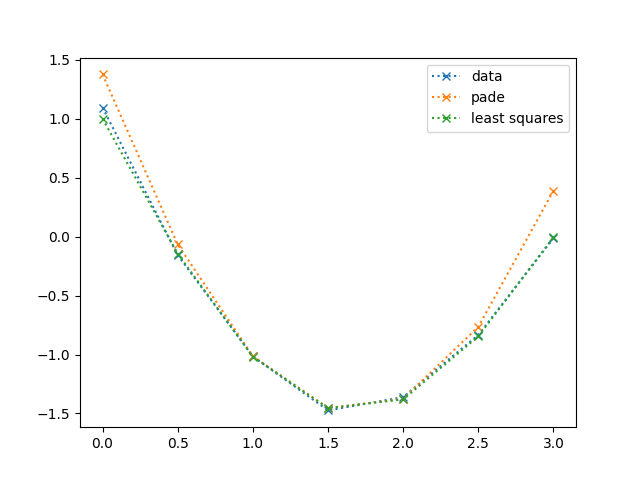
\includegraphics[width=\linewidth]{figures/compare_approx.png}
	\caption{Comparación de las aproximaciones}
	\label{fig:compare_approx}
\end{figure}

El error cuadrático, dado por:


$$
\text{SRR} = \sum_{k} (y_k - f(x_k))^2 
$$

es:
\begin{itemize}
	\item Padé: $0.254865$
	\item mínimos cuadrados: $0.010161$	
\end{itemize}

\subsection{Discusión}

Como es de esperar, la aproximación de Padé tiene mayor error que la de mínimos cuadrados, pero es aún una muy buena aproximación en la proximidad de $t_0$.

\begin{figure}[H]
	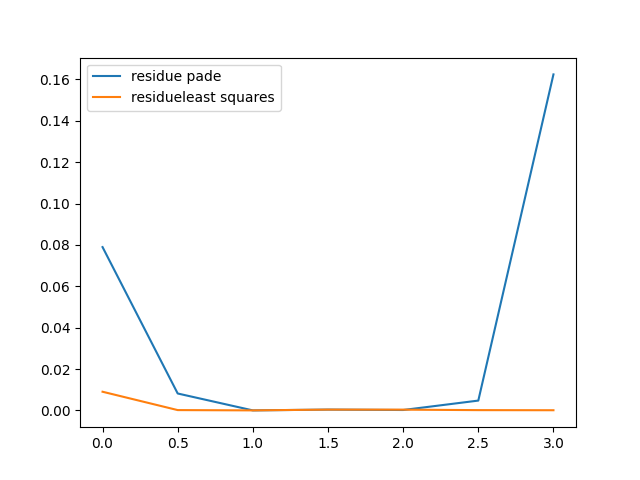
\includegraphics[width=\linewidth]{figures/errores_quad_approx.png}
	\caption{Error de las aproximaciones}
	\label{fig:error_quad_approx}
\end{figure}
\newpage 

% ejercicio F
\section{Error en la aproximación de Padé}

\subsection{Problema}
En relación a la función de ajuste $D(t)$ calculada por mínimos cuadrados, obtenga la funcióde error absoluto que se comete con el aproximante de Padédel apartado a) calculado alrededor de tres puntos distintos $t_0 = 1.0$, $t_0 = 1.5$ y $t_0 = 2.0$ y para los valores $\alpha$ y $\beta$ calculados en el ajuste. Calcule el error cuadrático en todos los casos y discuta la bondad de los ajustes.


\subsection{Resolución}

El código que se ha usado en la resolución de este problema está en \ref{code:ex6}. Se puede ver gráficamente el error absoluto de las tres aproximaciones en respecto al ajuste de mínimos cuadrados.

\begin{figure}[H]
	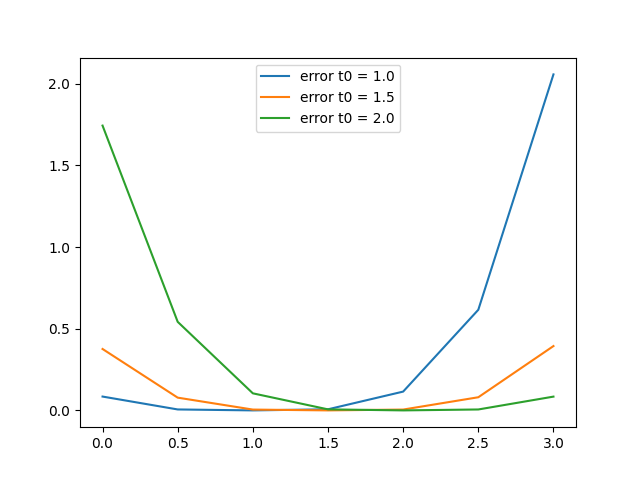
\includegraphics[width=\linewidth]{figures/error_abs_pade.png}
	\caption{Error de las aproximaciones de Padé en respecto al ajuste de mínimos cuadrados.}
	\label{fig:error_abs_pade}
\end{figure}

\newpage 

% ejercicio G
\section{Serie de Taylor}

\subsection{Problema}
Obtenga la expresión del desarrollo de Taylor de tercer grado para la función $D(t)$
dada al inicio del enunciado alrededor de un $t_0$ arbitrario. Particularice a los valores 
$t0 = 1.5$ y $\alpha$, $\beta$ calculados en el ajuste.

Calcule el error cuadrático que cometemos con el desarrollo de Taylor a la hora
de representar la tendencia de los datos experimentales.

Con respecto a la mejor función de ajuste $D(t)$ calculada por mínimos cuadrados,
calcule dos funciones de error: el error absoluto que se comete con este desarrollo de
Taylor y el error absoluto que se comete con el aproximante de Padé desarrollado
en torno a $t0 = 1.5$. Represente en una misma gráfica estas funciones de error y
extraiga las conclusiones.

\subsection{Resolución}

El código usado en este apartado se encuentra en \ref{code:ex7}.

\paragraph{Serie de Taylor de tercer grado}
Por suerte, ya hemos conseguido formular los coeficientes $a_k$ en relación a $t_0$, $\alpha$ y $\beta$ en el apartado a):

\begin{align*}
	&a_0 = D(t=t_0)  = e^{-\alpha t_0} + \beta \sin(t_0)
	= -1.4542154676453911 \\
&a_1 = \frac{\partial_t D(t=t_0)}{1!} 
= -\alpha e^{-\alpha t_0} + \beta \cos(t_0) 
= -0.36587527738259407\\
&a_2 = \frac{\partial_t^2 D(t=t_0)}{2!}
= \frac{\alpha^2 e^{-\alpha t_0} - \beta \sin(t_0)}{2}
= 1.0380572661767213\\
&a_3 = \frac{\partial_t^3 D(t=t_0)}{3!}
= \frac{-\alpha^3 e^{-\alpha t_0} - \beta \cos(t_0)}{6}	
= 0.01645851406923273
\end{align*}

y tenemos que la serie de Taylor de tercer grado es: 

$$
\sum_{k=0}^{3} a_k (t - t_0)^k = \sum_{k=0}^{3} a_k (t - 1.5)^k
$$

\newpage 

\paragraph{Ajuste de la serie de Taylor de tercer grado}
Podemos ver como se ajusta a los datos:

\begin{figure}[H]
	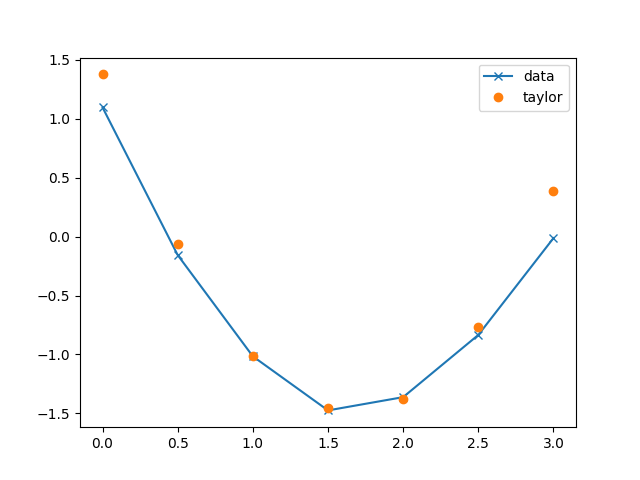
\includegraphics[width=\linewidth]{figures/taylor_expansion.png}
	\caption{Serie de Taylor de tercer grado}
	\label{fig:taylor_3rd_deg}
\end{figure}

\newpage 

\paragraph{Error cuadrático de la serie de Taylor de tercer grado}

El error cuadrático es $0.25296971634620236$ y se puede ver en la gráfica de abajo: 


\begin{figure}[H]
	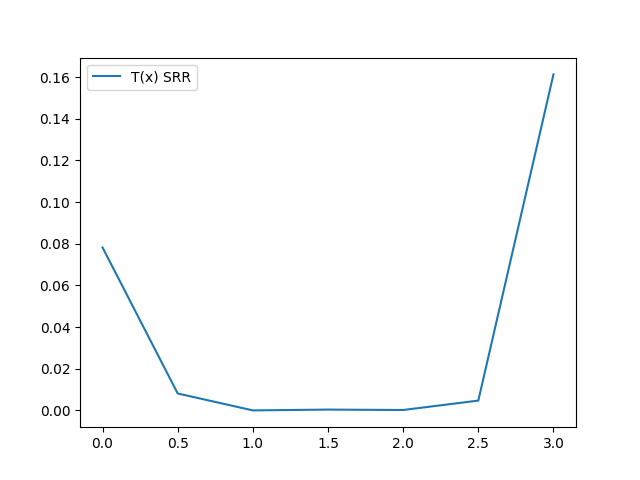
\includegraphics[width=\linewidth]{figures/taylor_quad_err.png}
	\caption{Error cuadrático de la serie de Taylor de tercer grado}
	\label{fig:taylor_3rd_deg_quad_err}
\end{figure}

\newpage 

\paragraph{Errores en respecto al ajuste por mínimos cuadrados}

Ahora procederemos a calcular y representar dos tipos de errores:

$$
S = \sum |y_k - f(x_k)|
$$

y 

$$
SRR = \sum (y_k - f(x_k))^2 
$$

donde la función $f(x_k)$ es la de ajuste por mínimos cuadrados usando los parámetros hallados en el apartado c). Haremos esto por cada aproximación.


\begin{figure}[H]
	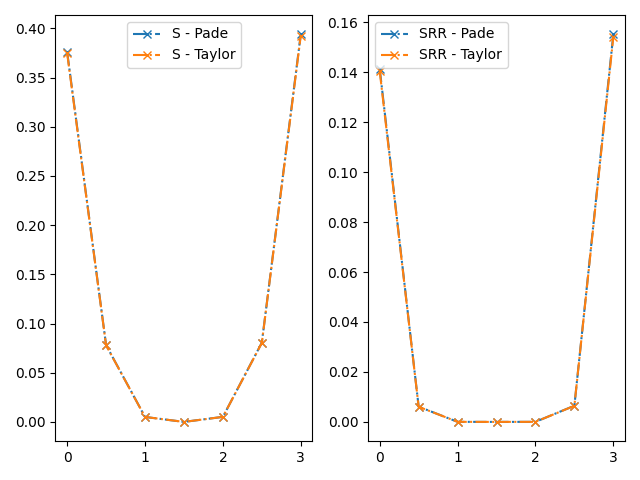
\includegraphics[width=\linewidth]{figures/approximation_errors.png}
	\caption{Errores en las aproximaciones}
	\label{fig:approximation_errors}
\end{figure}

Y los errores son:

\begin{itemize}
\item S - Pade: 0.938547
\item S - Taylor: 0.935348 
\item SRR - Pade: 0.309100 
\item SRR - Taylor: 0.306984 
\end{itemize}

\newpage 

\subsection{Discusión}

Lo primero de todo es que el error es mínimo cerca del punto de expansión $t_0 = 1.5$. Como hemos visto repetidamente en esta PEC, escoger bien el punto en torno al cual realizamos la aproximación es crucial. Segundo, la diferencia entre los errores es mínima, que muestra lo bueno que es el aproximante de Padé al ser de grado cuadrático en vez de cúbico como la aproximación de Taylor. Lo mas probable es que si tengamos que interpolar sobre un rango bastante amplio, se prefiera el aproximante de Padé al ser más estable mientras que el de Taylor es más fácil de calcular por ende mejor si el rango es un pequeño vecindario en torno al punto de expansión.
\newpage

\section{Apéndice}

\subsection{Código linalg}
\label{code:linalg}

\lstinputlisting[language=Python]{../../code/methods/linalg.py}


\subsection{Código datos}
\label{code:datos}

\lstinputlisting[language=Python]{../../code/pecs/pec4/data.py}

\subsection{Código Ejercicio C}
\label{code:ex3}

\lstinputlisting[language=Python]{../../code/pecs/pec4/ex3.py}

\subsection{Código Ejercicio D}
\label{code:ex4}

\lstinputlisting[language=Python]{../../code/pecs/pec4/ex4.py}

\subsection{Código Ejercicio E}
\label{code:ex5}

\lstinputlisting[language=Python]{../../code/pecs/pec4/ex5.py}

\subsection{Código Ejercicio F}
\label{code:ex6}

\lstinputlisting[language=Python]{../../code/pecs/pec4/ex6.py}

\subsection{Código Ejercicio G}
\label{code:ex7}

\lstinputlisting[language=Python]{../../code/pecs/pec4/ex7.py}
\newpage

\end{document}
